% Inbuilt themes in beamer
\documentclass[aspectratio=169]{beamer}

% Theme choice:
\usetheme[height=0.7cm, width=3cm]{Berkeley}
% 1. Change the main theme color (affects header, sidebar, and block titles)
\usecolortheme[named=black]{structure}
\setbeamercolor{title}{fg=black, bg=white}
\setbeamercolor{frametitle}{bg=lightgray, fg=black}     % Top header bar background & text
\setbeamercolor{sidebar}{bg=lightgray}                  % Left sidebar background
\setbeamercolor{logo}{bg=darkgray}                      % Top-left corner box (above sidebar)
\setbeamercolor{section in sidebar}{fg=black}           % Active section text in sidebar
\setbeamercolor{section in sidebar shaded}{fg=gray}     % Inactive section text in sidebar
\setbeamercolor{subsection in sidebar}{fg=black}        % Active subsection text
\setbeamercolor{subsection in sidebar shaded}{fg=gray}  % Inactive subsection text (use gray or darkgray)

% Adjust font sizes for sidebar elements
\setbeamerfont{title}{size=\LARGE, series=\bfseries}
\setbeamerfont{frametitle}{size=\normalsize, series=\bfseries}
\setbeamerfont{section in sidebar}{size=\normalsize, series=\bfseries}
\setbeamerfont{subsection in sidebar}{size=\scriptsize, series=\bfseries}

% Title page details: 
\title[]{\textbf{Introduction}} 
\author{}
\date{}


\begin{document}

% Title page frame
\begingroup
\makeatletter
\setlength{\hoffset}{-.5\beamer@sidebarwidth}
\makeatother
\begin{frame}[plain]
    \titlepage 
\end{frame}
\endgroup

% Outline frame
\begin{frame}[plain]{Outline}
    \tableofcontents
\end{frame}

% Frames
\section{Background}
\begin{frame}{Background}
    \begin{block}{Mathematics}
        Basic algebra
    \end{block}
    \begin{block}{Tools}
        \begin{itemize}
            \item Basic calculator
            \item Your brain
        \end{itemize}
    \end{block}
    \begin{alertblock}{Definition}
        Discrete structures are objects made of \underline{countable} elements.
    \end{alertblock}
\end{frame}

\section{Topics}
\subsection{Logic}
\begin{frame}{Logic}
    \begin{exampleblock}{Question}
        What language that machines understand?
    \end{exampleblock}

    \begin{figure}[h]
        \centering
        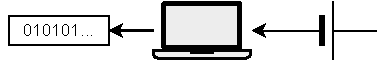
\includegraphics[width=0.6\textwidth]{images/01.computer.pdf}
    \end{figure}
    
    \begin{exampleblock}{Question}
        \begin{itemize}
            \item Since sugary soda is unhealthy, should we go with zero-sugar?
            \item Since great restaurants are always packed, should we just pick a crowded spot?
        \end{itemize}
    \end{exampleblock}
\end{frame}

\begin{frame}{Logic}
    \begin{exampleblock}{Question}
        If I forgot to bring my umbrella, then I'll get wet walking under the rain. Can we prove it? How many ways can we prove it?
    \end{exampleblock}

    \begin{exampleblock}{Question}
        For some certain conditions, 2 = 1. Is it true?
        \\
        \
        \\
        $a = b$ $\Rightarrow$ $a^2 = ab$ $\Rightarrow$ $a^2 - b^2 = ab - b^2$ $\Rightarrow$ $(a-b)(a+b) = b(a-b)$ $\Rightarrow$ $a+b = b$ $\Rightarrow$ $b+b = b$ $\Rightarrow$ $2b = b$ $\Rightarrow$ $2 = 1$
    \end{exampleblock}

    \begin{alertblock}{Definition}
        Logic is a two-state system: 0/1, True/False, On/Off, Yes/No, ...
    \end{alertblock}
\end{frame}

\subsection{Algorithms}
\begin{frame}{Induction}
    \begin{exampleblock}{Question}
        Imagine you have to prove that a statement is true for all natural numbers. Would you prove it one by one? Can you think of a more efficient way?
    \end{exampleblock}
    
    \begin{columns}[c]
        \begin{column}{0.7\textwidth}
            \begin{block}{Domino Effect}
                Imagine an infinitely long line of standing dominoes. You don't want to push every domino yourself. What is the smallest amount of work you can do to guarantee they all fall?
            \end{block}
        \end{column}
        \begin{column}{0.25\textwidth}
            \centering
            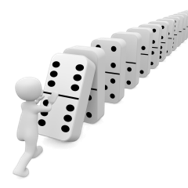
\includegraphics[width=\linewidth]{images/02.domino}
        \end{column}
    \end{columns}

    \begin{alertblock}{Definition}
        Induction is a proof method that simulates the domino effect.
    \end{alertblock}
\end{frame}

\begin{frame}{Recursion}
    \begin{exampleblock}{Question}
        Imagine you have to solve this complicated puzzle. What is your first step?
    \end{exampleblock}

    \begin{figure}
        \centering
        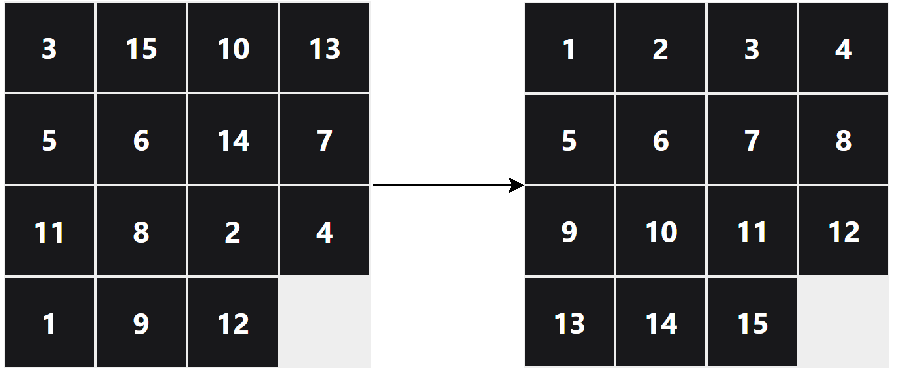
\includegraphics[width=0.6\textwidth]{images/03.sliding_puzzle}
    \end{figure}

    \begin{alertblock}{Definition}
        Recursion is a self-referential method that solves a problem by breaking it down into smaller subproblems.
    \end{alertblock}
    
\end{frame}

\subsection{Relations}
\begin{frame}{Relations}
    \begin{exampleblock}{Question}
        In the same network, do different devices have the unique IP address?
    \end{exampleblock}

    \begin{exampleblock}{Question}
        Secure transportation of information is a critical issue. How can we ensure that the information is not tampered with during transmission?
    \end{exampleblock}

    \begin{alertblock}{Definition}
        A relation is a set of ordered pairs. From a relation, we can use it to apply into real-world applications.
    \end{alertblock}
\end{frame}

\subsection{Counting and Probability}
\begin{frame}{Counting and Probability}
    \begin{exampleblock}{Question}
        We go to a ice cream shop and there are 4 flavors: vanilla, chocolate, strawberry and mint. How many different ways can we choose 2 scoops of ice cream?
    \end{exampleblock}

    \begin{exampleblock}{Question}
        In a gambling game, can we actually win the game? How can we calculate the probability of winning?
    \end{exampleblock}

    \begin{alertblock}{Definition}
        Counting and probability are fundamental concepts in discrete mathematics that help us analyze outcomes.
    \end{alertblock}
\end{frame}

\subsection{Graphs}
\begin{frame}{Graphs}
    \begin{exampleblock}{Question}
        How can Navigation apps find the shortest path from one location to another?
    \end{exampleblock}

    \begin{exampleblock}{Question}
        How social media can recommend a likely friend to you?
    \end{exampleblock}

    \begin{alertblock}{Definition}
        Graphs are structures that represent relationships between objects.
    \end{alertblock}
    
\end{frame}

\end{document}